\documentclass[twoside]{book}

% Packages required by doxygen
\usepackage{calc}
\usepackage{doxygen}
\usepackage{graphicx}
\usepackage[utf8]{inputenc}
\usepackage{makeidx}
\usepackage{multicol}
\usepackage{multirow}
\usepackage{fixltx2e}
\PassOptionsToPackage{warn}{textcomp}
\usepackage{textcomp}
\usepackage[nointegrals]{wasysym}
\usepackage[table]{xcolor}

% Font selection
\usepackage[T1]{fontenc}
\usepackage{mathptmx}
\usepackage[scaled=.90]{helvet}
\usepackage{courier}
\usepackage{amssymb}
\usepackage{sectsty}
\renewcommand{\familydefault}{\sfdefault}
\allsectionsfont{%
  \fontseries{bc}\selectfont%
  \color{darkgray}%
}
\renewcommand{\DoxyLabelFont}{%
  \fontseries{bc}\selectfont%
  \color{darkgray}%
}
\newcommand{\+}{\discretionary{\mbox{\scriptsize$\hookleftarrow$}}{}{}}

% Page & text layout
\usepackage{geometry}
\geometry{%
  a4paper,%
  top=2.5cm,%
  bottom=2.5cm,%
  left=2.5cm,%
  right=2.5cm%
}
\tolerance=750
\hfuzz=15pt
\hbadness=750
\setlength{\emergencystretch}{15pt}
\setlength{\parindent}{0cm}
\setlength{\parskip}{0.2cm}
\makeatletter
\renewcommand{\paragraph}{%
  \@startsection{paragraph}{4}{0ex}{-1.0ex}{1.0ex}{%
    \normalfont\normalsize\bfseries\SS@parafont%
  }%
}
\renewcommand{\subparagraph}{%
  \@startsection{subparagraph}{5}{0ex}{-1.0ex}{1.0ex}{%
    \normalfont\normalsize\bfseries\SS@subparafont%
  }%
}
\makeatother

% Headers & footers
\usepackage{fancyhdr}
\pagestyle{fancyplain}
\fancyhead[LE]{\fancyplain{}{\bfseries\thepage}}
\fancyhead[CE]{\fancyplain{}{}}
\fancyhead[RE]{\fancyplain{}{\bfseries\leftmark}}
\fancyhead[LO]{\fancyplain{}{\bfseries\rightmark}}
\fancyhead[CO]{\fancyplain{}{}}
\fancyhead[RO]{\fancyplain{}{\bfseries\thepage}}
\fancyfoot[LE]{\fancyplain{}{}}
\fancyfoot[CE]{\fancyplain{}{}}
\fancyfoot[RE]{\fancyplain{}{\bfseries\scriptsize Generated on Thu Jul 17 2014 00\+:28\+:31 for Zelda\+Oracle by Doxygen }}
\fancyfoot[LO]{\fancyplain{}{\bfseries\scriptsize Generated on Thu Jul 17 2014 00\+:28\+:31 for Zelda\+Oracle by Doxygen }}
\fancyfoot[CO]{\fancyplain{}{}}
\fancyfoot[RO]{\fancyplain{}{}}
\renewcommand{\footrulewidth}{0.4pt}
\renewcommand{\chaptermark}[1]{%
  \markboth{#1}{}%
}
\renewcommand{\sectionmark}[1]{%
  \markright{\thesection\ #1}%
}

% Indices & bibliography
\usepackage{natbib}
\usepackage[titles]{tocloft}
\setcounter{tocdepth}{3}
\setcounter{secnumdepth}{5}
\makeindex

% Hyperlinks (required, but should be loaded last)
\usepackage{ifpdf}
\ifpdf
  \usepackage[pdftex,pagebackref=true]{hyperref}
\else
  \usepackage[ps2pdf,pagebackref=true]{hyperref}
\fi
\hypersetup{%
  colorlinks=true,%
  linkcolor=blue,%
  citecolor=blue,%
  unicode%
}

% Custom commands
\newcommand{\clearemptydoublepage}{%
  \newpage{\pagestyle{empty}\cleardoublepage}%
}


%===== C O N T E N T S =====

\begin{document}

% Titlepage & ToC
\hypersetup{pageanchor=false,
             bookmarks=true,
             bookmarksnumbered=true,
             pdfencoding=unicode
            }
\pagenumbering{roman}
\begin{titlepage}
\vspace*{7cm}
\begin{center}%
{\Large Zelda\+Oracle }\\
\vspace*{1cm}
{\large Generated by Doxygen 1.8.7}\\
\vspace*{0.5cm}
{\small Thu Jul 17 2014 00:28:31}\\
\end{center}
\end{titlepage}
\clearemptydoublepage
\tableofcontents
\clearemptydoublepage
\pagenumbering{arabic}
\hypersetup{pageanchor=true}

%--- Begin generated contents ---
\chapter{Hierarchical Index}
\section{Class Hierarchy}
This inheritance list is sorted roughly, but not completely, alphabetically\+:\begin{DoxyCompactList}
\item \contentsline{section}{Door}{\pageref{structDoor}}{}
\item \contentsline{section}{Game}{\pageref{classGame}}{}
\item \contentsline{section}{Map}{\pageref{classMap}}{}
\item \contentsline{section}{Sprite}{\pageref{classSprite}}{}
\begin{DoxyCompactList}
\item \contentsline{section}{Character}{\pageref{classCharacter}}{}
\begin{DoxyCompactList}
\item \contentsline{section}{Player}{\pageref{classPlayer}}{}
\end{DoxyCompactList}
\end{DoxyCompactList}
\item \contentsline{section}{Sprite\+Animation}{\pageref{structSpriteAnimation}}{}
\item \contentsline{section}{Tileset}{\pageref{structTileset}}{}
\item \contentsline{section}{Timer}{\pageref{classTimer}}{}
\end{DoxyCompactList}

\chapter{Class Index}
\section{Class List}
Here are the classes, structs, unions and interfaces with brief descriptions\+:\begin{DoxyCompactList}
\item\contentsline{section}{\hyperlink{classCharacter}{Character} }{\pageref{classCharacter}}{}
\item\contentsline{section}{\hyperlink{structDoor}{Door} }{\pageref{structDoor}}{}
\item\contentsline{section}{\hyperlink{classGame}{Game} }{\pageref{classGame}}{}
\item\contentsline{section}{\hyperlink{classMap}{Map} }{\pageref{classMap}}{}
\item\contentsline{section}{\hyperlink{classPlayer}{Player} }{\pageref{classPlayer}}{}
\item\contentsline{section}{\hyperlink{classSprite}{Sprite} }{\pageref{classSprite}}{}
\item\contentsline{section}{\hyperlink{structSpriteAnimation}{Sprite\+Animation} }{\pageref{structSpriteAnimation}}{}
\item\contentsline{section}{\hyperlink{structTileset}{Tileset} }{\pageref{structTileset}}{}
\item\contentsline{section}{\hyperlink{classTimer}{Timer} }{\pageref{classTimer}}{}
\end{DoxyCompactList}

\chapter{Class Documentation}
\hypertarget{classCharacter}{\section{Character Class Reference}
\label{classCharacter}\index{Character@{Character}}
}
Inheritance diagram for Character\+:\begin{figure}[H]
\begin{center}
\leavevmode
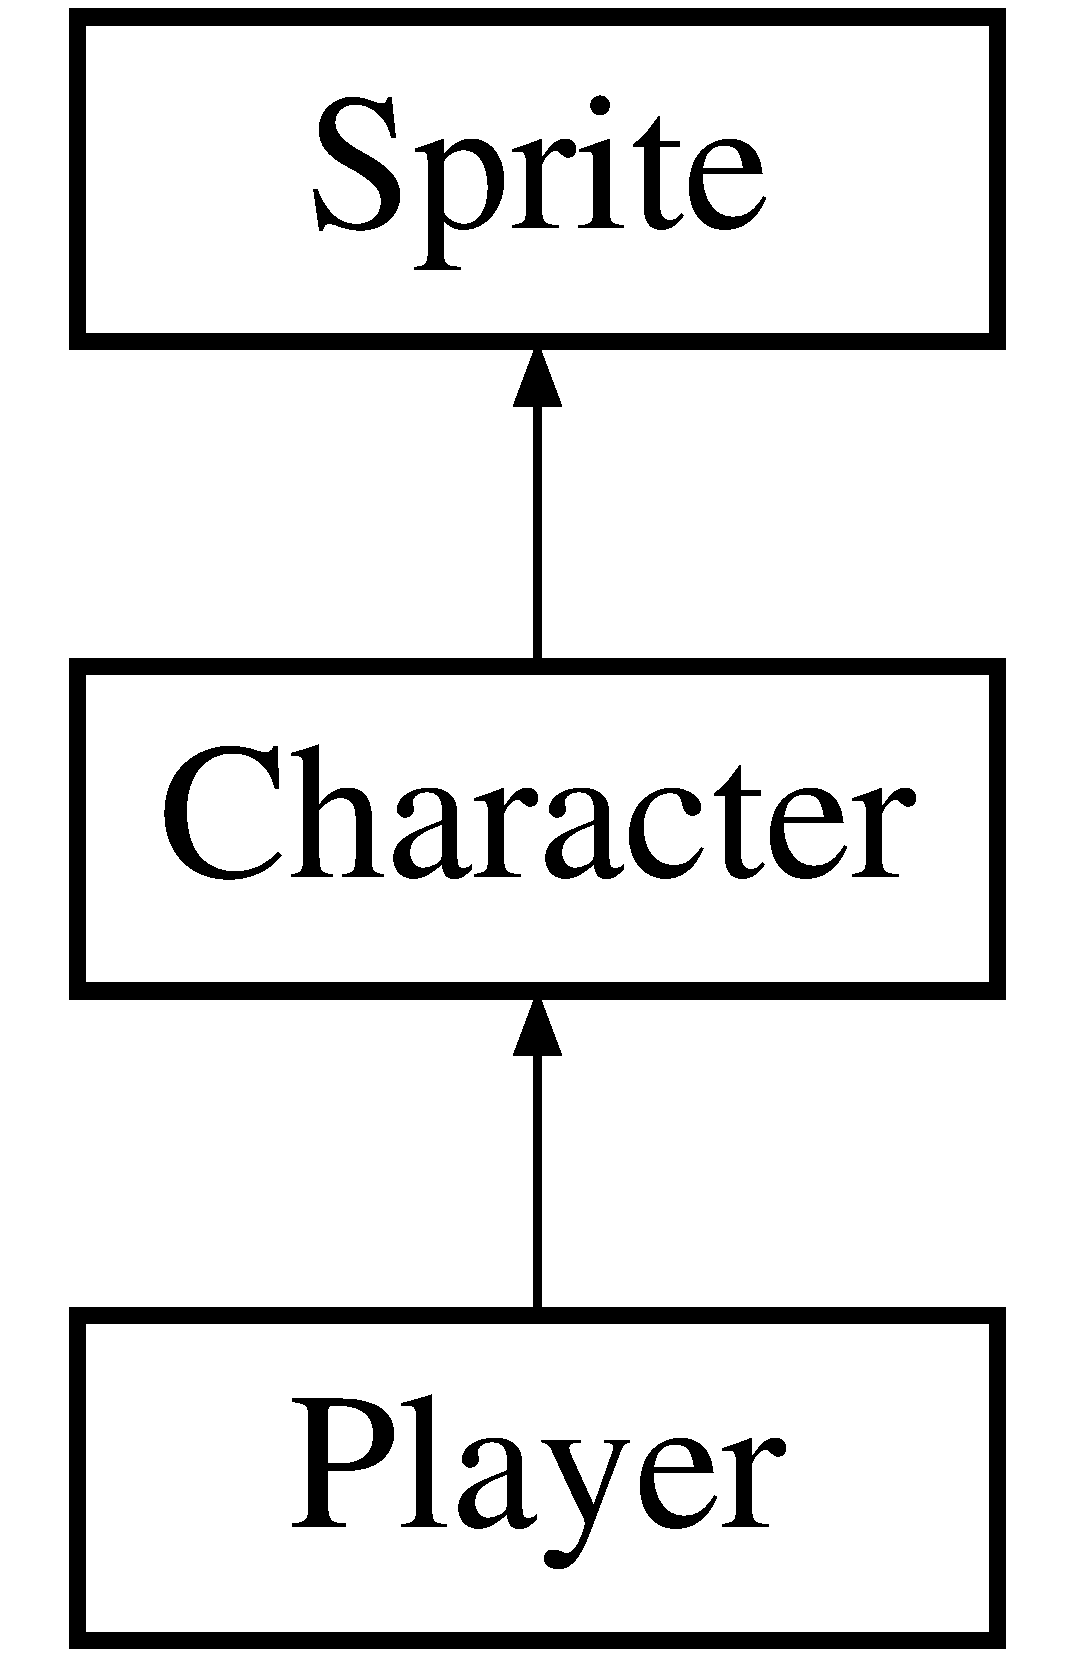
\includegraphics[height=3.000000cm]{classCharacter}
\end{center}
\end{figure}
\subsection*{Public Types}
\begin{DoxyCompactItemize}
\item 
\hypertarget{classCharacter_a0ee8f654ac7fbd527d0f64441cfc50ea}{enum {\bfseries Direction} \{ {\bfseries Down}, 
{\bfseries Right}, 
{\bfseries Left}, 
{\bfseries Up}
 \}}\label{classCharacter_a0ee8f654ac7fbd527d0f64441cfc50ea}

\end{DoxyCompactItemize}
\subsection*{Public Member Functions}
\begin{DoxyCompactItemize}
\item 
\hypertarget{classCharacter_a091f2955cac2fc5ae17af8013f4eb852}{{\bfseries Character} (u8 screen, s16 x, s16 y, u8 direction, u8 id, s5\+\_\+dimension size, u8 base\+Tile, u16 tile\+Size, u16 nb\+Tiles, u8 palette\+Slot, const void $\ast$tiles\+Data, const void $\ast$pal\+Data)}\label{classCharacter_a091f2955cac2fc5ae17af8013f4eb852}

\item 
\hypertarget{classCharacter_a45a63f9c964bc8286f691fa3eec7ad77}{void {\bfseries draw} ()}\label{classCharacter_a45a63f9c964bc8286f691fa3eec7ad77}

\item 
\hypertarget{classCharacter_a0f8b3a43420b0fda18d7898bdfca4c2a}{void {\bfseries test\+Collisions} ()}\label{classCharacter_a0f8b3a43420b0fda18d7898bdfca4c2a}

\item 
\hypertarget{classCharacter_a03a3141917ed01abbc72f4c057593bca}{void {\bfseries map\+Collisions} ()}\label{classCharacter_a03a3141917ed01abbc72f4c057593bca}

\item 
\hypertarget{classCharacter_a5dbb3462c702f6a9868dece29d45577e}{s16 {\bfseries x} () const }\label{classCharacter_a5dbb3462c702f6a9868dece29d45577e}

\item 
\hypertarget{classCharacter_a08197f0e29e3f9205bb2d222892ace20}{s16 {\bfseries y} () const }\label{classCharacter_a08197f0e29e3f9205bb2d222892ace20}

\item 
\hypertarget{classCharacter_a779caba22388ce362606de54b0aa339d}{void {\bfseries x} (s16 x)}\label{classCharacter_a779caba22388ce362606de54b0aa339d}

\item 
\hypertarget{classCharacter_a256a7f5bdb12bc7a4290cbddb37a9c24}{void {\bfseries y} (s16 y)}\label{classCharacter_a256a7f5bdb12bc7a4290cbddb37a9c24}

\item 
\hypertarget{classCharacter_a634313e1305254c233a0d40f513eac0f}{void {\bfseries vx} (s8 vx)}\label{classCharacter_a634313e1305254c233a0d40f513eac0f}

\item 
\hypertarget{classCharacter_a48707c906c6fd3cc4327aa71479cc7f0}{void {\bfseries vy} (s8 vy)}\label{classCharacter_a48707c906c6fd3cc4327aa71479cc7f0}

\end{DoxyCompactItemize}
\subsection*{Protected Attributes}
\begin{DoxyCompactItemize}
\item 
\hypertarget{classCharacter_ad0d297ed41044792f3144e98d361ef24}{float {\bfseries m\+\_\+x}}\label{classCharacter_ad0d297ed41044792f3144e98d361ef24}

\item 
\hypertarget{classCharacter_a7d65a136340c377b408808f9763a75a2}{float {\bfseries m\+\_\+y}}\label{classCharacter_a7d65a136340c377b408808f9763a75a2}

\item 
\hypertarget{classCharacter_a4cc303dcc38c81ac19c2820a60f5a33e}{float {\bfseries m\+\_\+vx}}\label{classCharacter_a4cc303dcc38c81ac19c2820a60f5a33e}

\item 
\hypertarget{classCharacter_ad173fd4b289f5c74ad81766cfc2ef2ac}{float {\bfseries m\+\_\+vy}}\label{classCharacter_ad173fd4b289f5c74ad81766cfc2ef2ac}

\item 
\hypertarget{classCharacter_a0e2c0871027ec614f2a7d4e283e9328f}{u8 {\bfseries m\+\_\+direction}}\label{classCharacter_a0e2c0871027ec614f2a7d4e283e9328f}

\item 
\hypertarget{classCharacter_aab07806fe827950f1b7a20be09b57ab9}{bool {\bfseries m\+\_\+moving}}\label{classCharacter_aab07806fe827950f1b7a20be09b57ab9}

\end{DoxyCompactItemize}


The documentation for this class was generated from the following files\+:\begin{DoxyCompactItemize}
\item 
/home/linux/\+Projects/\+Zelda\+Oracle/include/entities/Character.\+hpp\item 
/home/linux/\+Projects/\+Zelda\+Oracle/source/entities/Character.\+cpp\end{DoxyCompactItemize}

\hypertarget{structDoor}{\section{Door Struct Reference}
\label{structDoor}\index{Door@{Door}}
}
\subsection*{Public Member Functions}
\begin{DoxyCompactItemize}
\item 
\hypertarget{structDoor_a723f70412fbe3ded0805cde7d7371fdf}{{\bfseries Door} (u16 \+\_\+zone, u16 \+\_\+map\+X, u16 \+\_\+map\+Y, u16 \+\_\+spawn\+X, u16 \+\_\+spawn\+Y, u8 \+\_\+spawn\+Direction, u16 \+\_\+next\+Door\+I\+D)}\label{structDoor_a723f70412fbe3ded0805cde7d7371fdf}

\end{DoxyCompactItemize}
\subsection*{Public Attributes}
\begin{DoxyCompactItemize}
\item 
\hypertarget{structDoor_a62311e6c5ca163f59ee57c43a7bea4f6}{u16 {\bfseries zone}}\label{structDoor_a62311e6c5ca163f59ee57c43a7bea4f6}

\item 
\hypertarget{structDoor_a23761a863c0edd0844e069b4eb3b60a0}{u16 {\bfseries map\+X}}\label{structDoor_a23761a863c0edd0844e069b4eb3b60a0}

\item 
\hypertarget{structDoor_ace027e69fcd8dd0161a14727d0c9e5e4}{u16 {\bfseries map\+Y}}\label{structDoor_ace027e69fcd8dd0161a14727d0c9e5e4}

\item 
\hypertarget{structDoor_a2646b7b6376c3ec3089e9bc6b1c731a9}{u16 {\bfseries spawn\+X}}\label{structDoor_a2646b7b6376c3ec3089e9bc6b1c731a9}

\item 
\hypertarget{structDoor_acfad1de98748fcfaebd02415da9b6e05}{u16 {\bfseries spawn\+Y}}\label{structDoor_acfad1de98748fcfaebd02415da9b6e05}

\item 
\hypertarget{structDoor_a6efb884a2953fc77ba638ff4282da949}{u8 {\bfseries spawn\+Direction}}\label{structDoor_a6efb884a2953fc77ba638ff4282da949}

\item 
\hypertarget{structDoor_ab07bba0421e928507e98ac5619f966dc}{u16 {\bfseries next\+Door\+I\+D}}\label{structDoor_ab07bba0421e928507e98ac5619f966dc}

\end{DoxyCompactItemize}


The documentation for this struct was generated from the following file\+:\begin{DoxyCompactItemize}
\item 
/home/linux/\+Projects/\+Zelda\+Oracle/include/core/Door.\+hpp\end{DoxyCompactItemize}

\hypertarget{classGame}{\section{Game Class Reference}
\label{classGame}\index{Game@{Game}}
}
\subsection*{Public Member Functions}
\begin{DoxyCompactItemize}
\item 
\hypertarget{classGame_ac353a72ae342972b39efc7809de8fbfe}{void {\bfseries init\+Nitro\+F\+S} ()}\label{classGame_ac353a72ae342972b39efc7809de8fbfe}

\item 
\hypertarget{classGame_acfc5e19ef052dfade3c5a2eff31be13f}{void {\bfseries init\+Video} ()}\label{classGame_acfc5e19ef052dfade3c5a2eff31be13f}

\item 
\hypertarget{classGame_ab2e81e80929c807f557649522d8fbf00}{void {\bfseries init\+Sprite\+System} ()}\label{classGame_ab2e81e80929c807f557649522d8fbf00}

\item 
\hypertarget{classGame_ae89e277761b7dc5bc7a23fd1b4c6f17d}{void {\bfseries main\+Loop} ()}\label{classGame_ae89e277761b7dc5bc7a23fd1b4c6f17d}

\end{DoxyCompactItemize}


The documentation for this class was generated from the following files\+:\begin{DoxyCompactItemize}
\item 
/home/linux/\+Projects/\+Zelda\+Oracle/include/core/Game.\+hpp\item 
/home/linux/\+Projects/\+Zelda\+Oracle/source/core/Game.\+cpp\end{DoxyCompactItemize}

\hypertarget{classMap}{\section{Map Class Reference}
\label{classMap}\index{Map@{Map}}
}
\subsection*{Public Member Functions}
\begin{DoxyCompactItemize}
\item 
\hypertarget{classMap_a43109b24e3dbb3346e24f6f14de5c0b1}{{\bfseries Map} (\hyperlink{structTileset}{Tileset} $\ast$tileset, std\+::string filename, u16 width, u16 height, u16 zone, u16 x, u16 y)}\label{classMap_a43109b24e3dbb3346e24f6f14de5c0b1}

\item 
\hypertarget{classMap_a0c779ad064dcea5a8523962b3f0a3fd7}{u16 {\bfseries screen\+Pos} (s16 x, s16 y) const }\label{classMap_a0c779ad064dcea5a8523962b3f0a3fd7}

\item 
\hypertarget{classMap_a11fd1b88b5f3c923dad2c88df16e4373}{void {\bfseries load} ()}\label{classMap_a11fd1b88b5f3c923dad2c88df16e4373}

\item 
\hypertarget{classMap_a0c725b2b5aa05cbb6cd9555b9d40c4a9}{void {\bfseries load\+Tile} (s16 x, s16 y, s8 offset\+X=0, s8 offset\+Y=0)}\label{classMap_a0c725b2b5aa05cbb6cd9555b9d40c4a9}

\item 
\hypertarget{classMap_a6d1591e17d1d740102ea3d310b3bc691}{u16 {\bfseries get\+Tile} (u16 tile\+X, u16 tile\+Y)}\label{classMap_a6d1591e17d1d740102ea3d310b3bc691}

\item 
\hypertarget{classMap_a18f14d389c84ca7d8f75a0a31fdf35f7}{\hyperlink{structTileset}{Tileset} $\ast$ {\bfseries tileset} () const }\label{classMap_a18f14d389c84ca7d8f75a0a31fdf35f7}

\item 
\hypertarget{classMap_ab33fdb59d7aabee689251a8963410283}{u16 {\bfseries zone} () const }\label{classMap_ab33fdb59d7aabee689251a8963410283}

\item 
\hypertarget{classMap_a7427f72e828a67bd601ce3508d189fbe}{u16 {\bfseries x} () const }\label{classMap_a7427f72e828a67bd601ce3508d189fbe}

\item 
\hypertarget{classMap_a53215c2b905862830aab595fc09d63fb}{u16 {\bfseries y} () const }\label{classMap_a53215c2b905862830aab595fc09d63fb}

\end{DoxyCompactItemize}
\subsection*{Static Public Attributes}
\begin{DoxyCompactItemize}
\item 
\hypertarget{classMap_ab83915d4ac29e11a9c602551643d7bf4}{static s16 {\bfseries scroll\+X} = 0}\label{classMap_ab83915d4ac29e11a9c602551643d7bf4}

\item 
\hypertarget{classMap_a147fb969692ce9073350050018589f29}{static s16 {\bfseries scroll\+Y} = 0}\label{classMap_a147fb969692ce9073350050018589f29}

\end{DoxyCompactItemize}


The documentation for this class was generated from the following files\+:\begin{DoxyCompactItemize}
\item 
/home/linux/\+Projects/\+Zelda\+Oracle/include/display/Map.\+hpp\item 
/home/linux/\+Projects/\+Zelda\+Oracle/source/display/Map.\+cpp\end{DoxyCompactItemize}

\hypertarget{classPlayer}{\section{Player Class Reference}
\label{classPlayer}\index{Player@{Player}}
}
Inheritance diagram for Player\+:\begin{figure}[H]
\begin{center}
\leavevmode
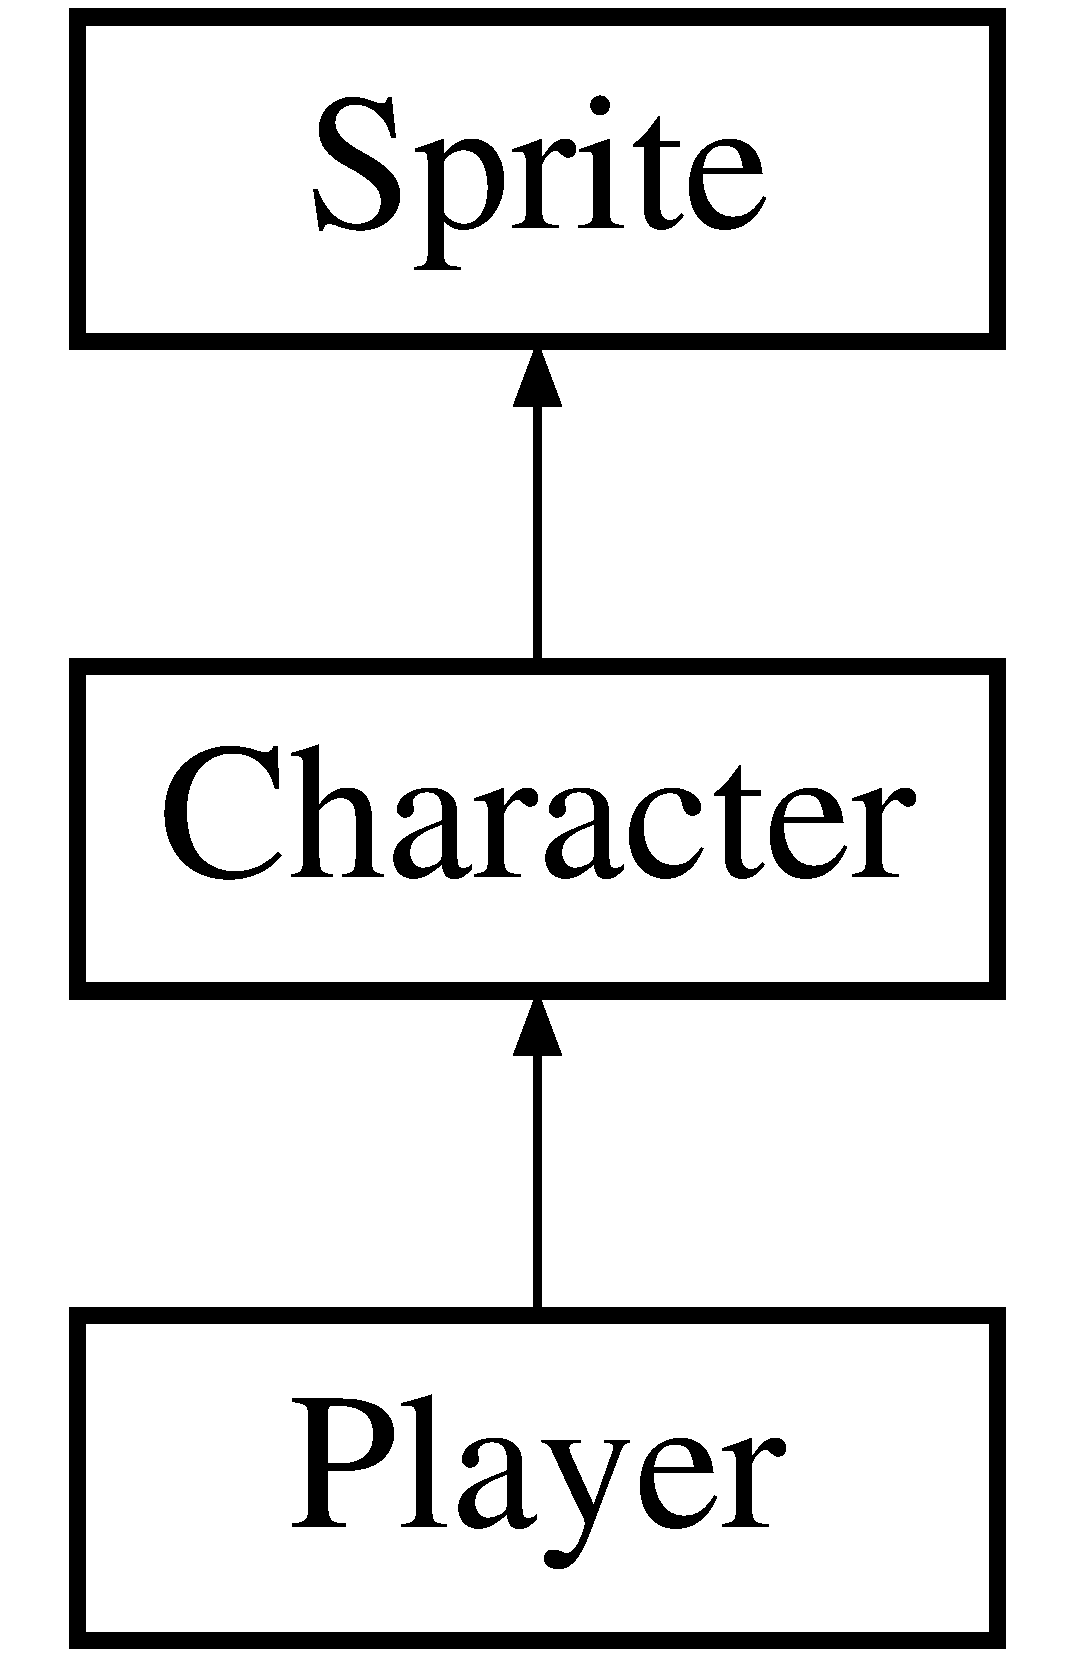
\includegraphics[height=3.000000cm]{classPlayer}
\end{center}
\end{figure}
\subsection*{Public Member Functions}
\begin{DoxyCompactItemize}
\item 
\hypertarget{classPlayer_a23d57e9f0d726e7510c911cc22c08eda}{void {\bfseries test\+Collisions} ()}\label{classPlayer_a23d57e9f0d726e7510c911cc22c08eda}

\item 
\hypertarget{classPlayer_a950759ed42b270061fb1e546ba4fa891}{void {\bfseries door\+Collisions} ()}\label{classPlayer_a950759ed42b270061fb1e546ba4fa891}

\item 
\hypertarget{classPlayer_ae02ee46d8c20dd0697b975f935b09839}{void {\bfseries move} ()}\label{classPlayer_ae02ee46d8c20dd0697b975f935b09839}

\end{DoxyCompactItemize}
\subsection*{Additional Inherited Members}


The documentation for this class was generated from the following files\+:\begin{DoxyCompactItemize}
\item 
/home/linux/\+Projects/\+Zelda\+Oracle/include/entities/Player.\+hpp\item 
/home/linux/\+Projects/\+Zelda\+Oracle/source/entities/Player.\+cpp\end{DoxyCompactItemize}

\hypertarget{classSprite}{\section{Sprite Class Reference}
\label{classSprite}\index{Sprite@{Sprite}}
}
Inheritance diagram for Sprite\+:\begin{figure}[H]
\begin{center}
\leavevmode
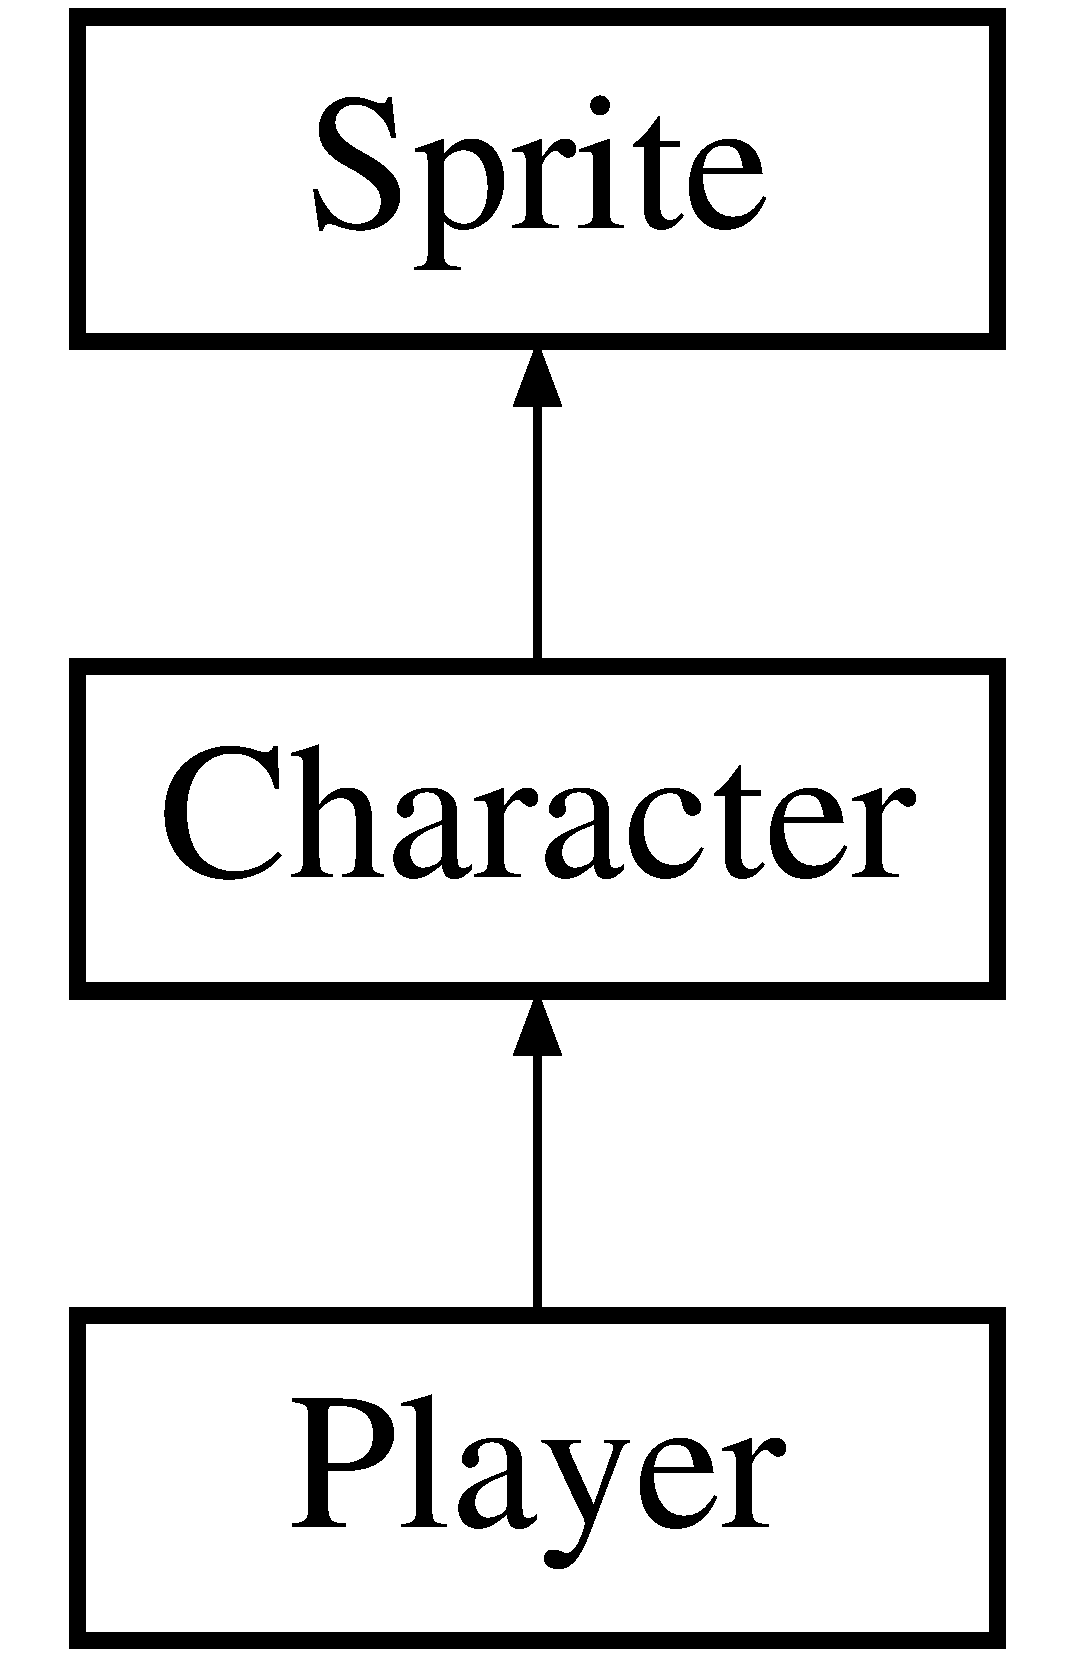
\includegraphics[height=3.000000cm]{classSprite}
\end{center}
\end{figure}
\subsection*{Public Member Functions}
\begin{DoxyCompactItemize}
\item 
\hypertarget{classSprite_af2a7c9959b01ec19a7875ac42bc24f6a}{{\bfseries Sprite} (u8 screen, u8 id, s5\+\_\+dimension size, u8 base\+Tile, u16 tile\+Size, u16 nb\+Tiles, u8 palette\+Slot, const void $\ast$tiles\+Data, const void $\ast$pal\+Data)}\label{classSprite_af2a7c9959b01ec19a7875ac42bc24f6a}

\item 
\hypertarget{classSprite_a36b20b1988778637e82ea71b03f24c36}{void {\bfseries clear} ()}\label{classSprite_a36b20b1988778637e82ea71b03f24c36}

\item 
\hypertarget{classSprite_aefebc6e7c004bead1aa144a47980f0c0}{void {\bfseries draw\+Frame} (s16 x, s16 y, u8 frame)}\label{classSprite_aefebc6e7c004bead1aa144a47980f0c0}

\item 
\hypertarget{classSprite_a43b4b5a1024d4dbf16ff06c1ce88fa00}{void {\bfseries add\+Animation} (u8 size, u8 $\ast$frames, u16 delay)}\label{classSprite_a43b4b5a1024d4dbf16ff06c1ce88fa00}

\item 
\hypertarget{classSprite_a8fc89150457a37d78ae7974acc2441ed}{void {\bfseries stop\+Animation} (u8 anim)}\label{classSprite_a8fc89150457a37d78ae7974acc2441ed}

\item 
\hypertarget{classSprite_afba1a990e82eb6bf2c1786b273a2d8d6}{void {\bfseries start\+Animation} (u8 anim)}\label{classSprite_afba1a990e82eb6bf2c1786b273a2d8d6}

\item 
\hypertarget{classSprite_a8dfa9b2c4801fce3cac536bd155728c6}{void {\bfseries reset\+Animation} (u8 anim)}\label{classSprite_a8dfa9b2c4801fce3cac536bd155728c6}

\item 
\hypertarget{classSprite_a619b3a4fdd0453fbaad622d2dde9d0b4}{bool {\bfseries is\+Animation\+At\+End} (u8 anim)}\label{classSprite_a619b3a4fdd0453fbaad622d2dde9d0b4}

\item 
\hypertarget{classSprite_a101944b94b6259e176318ba492d5acc6}{void {\bfseries play\+Animation} (s16 x, s16 y, u8 anim)}\label{classSprite_a101944b94b6259e176318ba492d5acc6}

\end{DoxyCompactItemize}
\subsection*{Protected Attributes}
\begin{DoxyCompactItemize}
\item 
\hypertarget{classSprite_a0563d59ccc4bf4f3ed47a9dea46c8b18}{u8 {\bfseries m\+\_\+screen}}\label{classSprite_a0563d59ccc4bf4f3ed47a9dea46c8b18}

\item 
\hypertarget{classSprite_a7b32e8dcd40a03954c3f2afd0b5a7d95}{u8 {\bfseries m\+\_\+id}}\label{classSprite_a7b32e8dcd40a03954c3f2afd0b5a7d95}

\item 
\hypertarget{classSprite_a1fbd3dd9bae872f5198fe23ff674d568}{s5\+\_\+dimension {\bfseries m\+\_\+size}}\label{classSprite_a1fbd3dd9bae872f5198fe23ff674d568}

\item 
\hypertarget{classSprite_a60aa50330a44abfb6defd4ef37c86044}{s5\+\_\+colors {\bfseries m\+\_\+color}}\label{classSprite_a60aa50330a44abfb6defd4ef37c86044}

\item 
\hypertarget{classSprite_a8a6cd96e1c882a0a6f39064c162c150a}{u8 {\bfseries m\+\_\+base\+Tile}}\label{classSprite_a8a6cd96e1c882a0a6f39064c162c150a}

\item 
\hypertarget{classSprite_ad9409d7e3de265d8a967a4ea7ccc9070}{u16 {\bfseries m\+\_\+tile\+Size}}\label{classSprite_ad9409d7e3de265d8a967a4ea7ccc9070}

\item 
\hypertarget{classSprite_acc78719792d7dc0d094ec08ac598e376}{u8 {\bfseries m\+\_\+palette\+Slot}}\label{classSprite_acc78719792d7dc0d094ec08ac598e376}

\item 
\hypertarget{classSprite_afed43cbdbec4fbdd8138844384e788ef}{std\+::vector$<$ \hyperlink{structSpriteAnimation}{Sprite\+Animation} $>$ {\bfseries m\+\_\+animations}}\label{classSprite_afed43cbdbec4fbdd8138844384e788ef}

\end{DoxyCompactItemize}


The documentation for this class was generated from the following files\+:\begin{DoxyCompactItemize}
\item 
/home/linux/\+Projects/\+Zelda\+Oracle/include/display/Sprite.\+hpp\item 
/home/linux/\+Projects/\+Zelda\+Oracle/source/display/Sprite.\+cpp\end{DoxyCompactItemize}

\hypertarget{structSpriteAnimation}{\section{Sprite\+Animation Struct Reference}
\label{structSpriteAnimation}\index{Sprite\+Animation@{Sprite\+Animation}}
}
\subsection*{Public Member Functions}
\begin{DoxyCompactItemize}
\item 
\hypertarget{structSpriteAnimation_a3ba301d059d8f247ea4c96d47a85768a}{{\bfseries Sprite\+Animation} (u16 \+\_\+size, u8 $\ast$\+\_\+tab\+Anim, u16 \+\_\+delay)}\label{structSpriteAnimation_a3ba301d059d8f247ea4c96d47a85768a}

\end{DoxyCompactItemize}
\subsection*{Public Attributes}
\begin{DoxyCompactItemize}
\item 
\hypertarget{structSpriteAnimation_aa547caf0c49262f082865ab9422619ea}{u16 {\bfseries size}}\label{structSpriteAnimation_aa547caf0c49262f082865ab9422619ea}

\item 
\hypertarget{structSpriteAnimation_a25b1c835bb1754c37db207ecfebfd7ce}{u8 $\ast$ {\bfseries tab\+Anim}}\label{structSpriteAnimation_a25b1c835bb1754c37db207ecfebfd7ce}

\item 
\hypertarget{structSpriteAnimation_a8692dae92b2f3f23fb27846fad397f98}{u16 {\bfseries delay}}\label{structSpriteAnimation_a8692dae92b2f3f23fb27846fad397f98}

\item 
\hypertarget{structSpriteAnimation_a7f051b8f289ffd16b226bc2abbd26888}{\hyperlink{classTimer}{Timer} {\bfseries timer}}\label{structSpriteAnimation_a7f051b8f289ffd16b226bc2abbd26888}

\item 
\hypertarget{structSpriteAnimation_a37b4a887ed53f1b808a37dad19083f0e}{bool {\bfseries is\+Playing}}\label{structSpriteAnimation_a37b4a887ed53f1b808a37dad19083f0e}

\end{DoxyCompactItemize}


The documentation for this struct was generated from the following file\+:\begin{DoxyCompactItemize}
\item 
/home/linux/\+Projects/\+Zelda\+Oracle/include/display/Sprite\+Animation.\+hpp\end{DoxyCompactItemize}

\hypertarget{structTileset}{\section{Tileset Struct Reference}
\label{structTileset}\index{Tileset@{Tileset}}
}
\subsection*{Public Member Functions}
\begin{DoxyCompactItemize}
\item 
\hypertarget{structTileset_a07a467452269b180d9648b8654ed4360}{{\bfseries Tileset} (u8 $\ast$\+\_\+info, const unsigned int $\ast$\+\_\+tiles, u32 \+\_\+tiles\+Length, const u16 $\ast$\+\_\+palette, u32 \+\_\+pal\+Length)}\label{structTileset_a07a467452269b180d9648b8654ed4360}

\end{DoxyCompactItemize}
\subsection*{Public Attributes}
\begin{DoxyCompactItemize}
\item 
\hypertarget{structTileset_acc283d7b507dd0c2fbd569adc5bdefc6}{u8 $\ast$ {\bfseries info}}\label{structTileset_acc283d7b507dd0c2fbd569adc5bdefc6}

\item 
\hypertarget{structTileset_a287ee4f9016e47dd67a93a8737b7ec75}{const unsigned int $\ast$ {\bfseries tiles}}\label{structTileset_a287ee4f9016e47dd67a93a8737b7ec75}

\item 
\hypertarget{structTileset_a4b2815f4c044a8a0a664d469f11286bf}{u32 {\bfseries tiles\+Length}}\label{structTileset_a4b2815f4c044a8a0a664d469f11286bf}

\item 
\hypertarget{structTileset_a1070f3d36c53f86ad5f42ddd2722c595}{const u16 $\ast$ {\bfseries palette}}\label{structTileset_a1070f3d36c53f86ad5f42ddd2722c595}

\item 
\hypertarget{structTileset_a038d33e6acfee0ec6c69e450232fd427}{u32 {\bfseries pal\+Length}}\label{structTileset_a038d33e6acfee0ec6c69e450232fd427}

\end{DoxyCompactItemize}


The documentation for this struct was generated from the following file\+:\begin{DoxyCompactItemize}
\item 
/home/linux/\+Projects/\+Zelda\+Oracle/include/display/Tileset.\+hpp\end{DoxyCompactItemize}

\hypertarget{classTimer}{\section{Timer Class Reference}
\label{classTimer}\index{Timer@{Timer}}
}
\subsection*{Public Member Functions}
\begin{DoxyCompactItemize}
\item 
\hypertarget{classTimer_a63f0eb44b27402196590a03781515dba}{void {\bfseries stop} ()}\label{classTimer_a63f0eb44b27402196590a03781515dba}

\item 
\hypertarget{classTimer_a3a8b5272198d029779dc9302a54305a8}{void {\bfseries start} ()}\label{classTimer_a3a8b5272198d029779dc9302a54305a8}

\item 
\hypertarget{classTimer_a9020542d73357a4eef512eefaf57524b}{void {\bfseries reset} ()}\label{classTimer_a9020542d73357a4eef512eefaf57524b}

\item 
\hypertarget{classTimer_a7715979fee128ff708344462375a169a}{u32 {\bfseries time} ()}\label{classTimer_a7715979fee128ff708344462375a169a}

\end{DoxyCompactItemize}
\subsection*{Static Public Member Functions}
\begin{DoxyCompactItemize}
\item 
\hypertarget{classTimer_af28f8e2d5ed47f8f18b2c61e549559bd}{static void {\bfseries init\+System\+Timer} ()}\label{classTimer_af28f8e2d5ed47f8f18b2c61e549559bd}

\end{DoxyCompactItemize}
\subsection*{Static Public Attributes}
\begin{DoxyCompactItemize}
\item 
\hypertarget{classTimer_a2754d03574ede5fbd1b496547cd8b47b}{static u32 {\bfseries system\+Time} = 0}\label{classTimer_a2754d03574ede5fbd1b496547cd8b47b}

\end{DoxyCompactItemize}


The documentation for this class was generated from the following files\+:\begin{DoxyCompactItemize}
\item 
/home/linux/\+Projects/\+Zelda\+Oracle/include/core/Timer.\+hpp\item 
/home/linux/\+Projects/\+Zelda\+Oracle/source/core/Timer.\+cpp\end{DoxyCompactItemize}

%--- End generated contents ---

% Index
\newpage
\phantomsection
\addcontentsline{toc}{chapter}{Index}
\printindex

\end{document}
